%% USPSC-modelo.tex
% ---------------------------------------------------------------
% USPSC: Modelo de Trabalho Academico (tese de doutorado, dissertacao de
% mestrado e trabalhos monograficos em geral) em conformidade com 
% ABNT NBR 14724:2011: Informacao e documentacao - Trabalhos academicos -
% Apresentacao
%----------------------------------------------------------------
%% Esta é uma customização do abntex2-modelo-trabalho-academico.tex de v-1.9.5 laurocesar 
%% para as Unidades do Campus USP de São Carlos:
%% EESC - Escola de Engenharia de São Carlos
%% IAU - Instituto de Arquitetura e Urbanismo
%% ICMC - Instituto de Ciências Matemáticas e de Computação
%% IFSC - Instituto de Física de São Carlos
%% IQSC - Instituto de Química de São Carlos
%%
%% Este trabalho utiliza a classe USPSC.cls que é mantida pela seguinte equipe:
%% 
%% Programação:
%%   - Marilza Aparecida Rodrigues Tognetti - marilza@sc.usp.br (PUSP-SC)
%%   - Ana Paula Aparecida Calabrez - aninha@sc.usp.br (PUSP-SC)
%% Normalização e Padronização:
%%   - Brianda de Oliveira Ordonho Sigolo - brianda@usp.br (IAU)
%%   - Elena Luzia Palloni Gonçalves - elena@sc.usp.br (EESC)
%%   - Eliana de Cássia Aquareli Cordeiro - eliana@iqsc.usp.br (IQSC)
%%   - Flávia Helena Cassin - cassinp@sc.usp.br (EESC)
%%   - Maria Cristina Cavarette Dziabas - mcdziaba@ifsc.usp.br (IFSC)
%%   - Regina Célia Vidal Medeiros - rcvmat@icmc.usp.br (ICMC)
%%
%% O USPSC-modelo.tex utiliza:	
%%  USPSC.cls e USPSC1.cls
%% 	USPSC-modelo-references.bib
%%	USPSC-modelo.tex
%%	USPSC-unidades.tex
%%	Um dos arquivos com dados pre-textuais abaixo, em conformidade com a Unidade de vínculo do autor:
%%				USPSC-pre-textual-EESC.tex
%%				USPSC-pre-textual-IAU.tex
%%				USPSC-pre-textual-ICMC.tex
%%				USPSC-pre-textual-IFSC.tex
%%				USPSC-pre-textual-IQSC.tex
%%				USPSC-pre-textual-OUTRO.tex
%%	USPSC-fichacatalografica.tex ou fichacatalografica.pdf
%%	folhadeaprovacao.pdf
%%	USPSC-Cap1-Introducao.tex
%%	USPSC-Cap2-Desenvolvimento.tex
%%	USPSC-Cap3-Citacoes.tex
%%	USPSC-Cap4-referencias.tex
%%	USPSC-Cap5-Conclusao.tex
%%	USPSC-Apendices.tex
%%	USPSC-Anexos.tex
%%	USPSC-AcentuacaoLaTeX.tex
%%	USPSC-LetrasGregas.tex
%%	USPSC-SimbolosUteis.tex

%----------------------------------------------------------------
%% Sobre a classe abntex2.cls:
%% abntex2.cls, v-1.9.5 laurocesar
%% Copyright 2012-2015 by abnTeX2 group at https://www.abntex.net.br/ 
%%
%----------------------------------------------------------------

\documentclass[
% -- opções da classe memoir --
12pt,		% tamanho da fonte
openright,	% capítulos começam em pág ímpar (insere página vazia caso preciso)
twoside,  % para impressão em anverso (frente) e verso. Oposto a oneside - Nota: utilizar \imprimirfolhaderosto*
%oneside, % para impressão em páginas separadas (somente anverso) -  Nota: utilizar \imprimirfolhaderosto
% inclua uma % antes do comando twoside e exclua a % antes do oneside 
a4paper,			% tamanho do papel. 
% -- opções da classe abntex2 --
chapter=TITLE,		% títulos de capítulos convertidos em letras maiúsculas
% -- opções do pacote babel --
english,			% idioma adicional para hifenização
french,				% idioma adicional para hifenização
spanish,			% idioma adicional para hifenização
brazil				% o último idioma é o principal do documento
% {USPSC} configura o cabeçalho contendo apenas o número da página
]{USPSC}
%]{USPSC1}
% Inclua % antes de ]{USPSC} e retire a % antes de %]{USPSC1}
% para utilizar o cabeçalho diferenciado para as páginas pares e ímpares como indicado abaixo:
%- páginas ímpares: cabeçalho com seções ou subseções e o número da página
%- páginas pares: cabeçalho com o número da página e o título do capítulo 
% ---

% ---
% Pacotes básicos - Fundamentais 
% ---
\usepackage[T1]{fontenc}		% Seleção de códigos de fonte.
\usepackage[utf8]{inputenc}		% Codificação do documento (conversão automática dos acentos)
\usepackage{lmodern}			% Usa a fonte Latin Modern
% Para utilizar a fonte Times New Roman, inclua uma % no início do comando acima  "\usepackage{lmodern}"
% Abaixo, tire a % antes do comando  \usepackage{times}
%\usepackage{times}		    	% Usa a fonte Times New Roman	
% Lembre-se de alterar a fonte no comando que imprime o preâmbulo no arquivo da Classe USPSC.cls				
\usepackage{lastpage}			% Usado pela Ficha catalográfica
\usepackage{indentfirst}		% Indenta o primeiro parágrafo de cada seção.
\usepackage{color}				% Controle das cores
\usepackage{graphicx}			% Inclusão de gráficos
\usepackage{float} 				% Fixa tabelas e figuras no local exato
\usepackage{chemfig,chemmacros} % Para escrever reações químicas
\usepackage{microtype} 			% para melhorias de justificação
\usepackage{pdfpages}
\usepackage{makeidx}            % para gerar índice remissimo
% ---

% ---
% Pacotes de citações
% Citações padrão ABNT
% ---
% Sistemas de chamada: autor-data ou numérico.
% Sistema autor-data
%\usepackage[alf,abnt-emphasize=bf, abnt-thesis-year=both, abnt-repeated-author-omit=yes, abnt-last-names=abnt, abnt-etal-cite,abnt-etal-list=3, abnt-etal-text=default, abnt-and-type=e, abnt-doi=doi, abnt-url-package=none, abnt-verbatim-entry=no]{abntex2cite}

% Para o IQSC, que indica todos os autores nas referências, incluir % no início do comando acima e retirar a % do comando abaixo 

%\usepackage[alf,abnt-emphasize=bf, abnt-thesis-year=both, abnt-repeated-author-omit=yes, abnt-last-names=abnt, abnt-etal-cite,abnt-etal-list=0, abnt-etal-text=default, abnt-and-type=e]{abntex2cite}

% Sistema Numérico
% Para citações numéricas, sistema adotado pelo IFSC, incluir % no início do comando acima e retirar a % do comando abaixo 
\usepackage[num,overcite,abnt-emphasize=bf, abnt-thesis-year=both, abnt-repeated-author-omit=yes, abnt-last-names=abnt, abnt-etal-cite,abnt-etal-list=0, abnt-etal-text=default, abnt-and-type=e]{abntex2cite}
% Complementarmente, verifique as instruções abaixo sobre os Pacotes de Nota de rodapé
% ---
% Pacotes de Nota de rodapé
% Configurações de nota de rodapé

% O presente modelo adota o formato numérico para as notas de rodapés quando utiliza o sistema de chamada autor-data para citações e referências. Para utilizar o sistema de chamada numérico para citações e referências, habilitar um dos comandos abaixo.
% Há diversa opções para nota de rodapé no Sistema Numérico.  Para o IFSC, habilitade o comando abaixo.

\renewcommand{\thefootnote}{\fnsymbol{footnote}}  %Comando para inserção de símbolos em nota de rodapé

% Outras opções para nota de rodapé no Sistema Numérico:
%\renewcommand{\thefootnote}{\alph{footnote}}      %Comando para inserção de letras minúscula em nota de rodapé
%\renewcommand{\thefootnote}{\Alph{footnote}}      %Comando para inserção de letras maiúscula em nota de rodapé
%\renewcommand{\thefootnote}{\roman{footnote}}     %Comando para inserção de números romanos minúsculos  em nota de rodapé
%\renewcommand{\thefootnote}{\Roman{footnote}}     %Comando para inserção de números romanos minúsculos  em nota de rodapé

\renewcommand{\footnotesize}{\small} %Comando para diminuir a fonte das notas de rodapé

 % ---
 % Pacote para agrupar a citação numérica consecutiva
 % Quando for adotado o Sistema Numérico, a exemplo do IFSC, habilite 
 % o pacote cite abaixo retirando a porcentagem antes do comando abaixo
 \usepackage[superscript]{cite}	

% ---
% Pacotes adicionais, usados apenas no âmbito do Modelo Canônico do abnteX2
% ---
\usepackage{lipsum}				% para geração de dummy text
% ---




% pacotes de tabelas
\usepackage{multicol}	% Suporte a mesclagens em colunas
\usepackage{multirow}	% Suporte a mesclagens em linhas
\usepackage{longtable}	% Tabelas com várias páginas
\usepackage{threeparttablex}    % notas no longtable
\usepackage{array}

%---
% Configurações para o pacote chemfig
%\chemsetup[chemformula]{format=\sffamily}
\renewcommand*\printatom[1]{\ensuremath{\mathsf{#1}}}
\setatomsep{2em}
\setdoublesep{.6ex}
\setbondstyle{semithick}
%---
% Configurando o ambiente para utilizar os recursos de frases pre-prontas do mhchem
\newenvironment{rslist}%
{%
	\begin{labeling}% environment from KOMA-script
		{\rsnumber{R39/23/24/25}}% R39/23/24/25 is longest label
	}{%
\end{labeling}%
}%
% Definição de comando para utilizar os recursos de frases pre-prontas do mhchem
\newcommand{\rs}[2][]{\item[{\rsnumber[#1]{#2}}] \rsphrase{bb}}
% ---

% ---
% DADOS INICIAIS - Define sigla com título, área de concentração e opção do Programa 
% Consulte a tabela referente aos Programas, áreas e opções de sua unidade contante do
% arquivo USPSC-Siglas estabelecidas para os Programas de Pós-Graduação por Unidade.xlsx 
% ou nos APÊNDICES A-E
\siglaunidade{IFSC}
\programa{DFAFC}
% Os demais dados deverão ser fornecidos no arquivo USPSC-pre-textual-UUUU, onde UUUU é a sigla da Unidade. 
% Exemplo:USPSC-pre-textual-IFSC.tex
% ---
% Configurações de aparência do PDF final
% alterando o aspecto da cor azul
\definecolor{blue}{RGB}{41,5,195}

% informações do PDF
\makeatletter
\hypersetup{
	%pagebackref=true,
	pdftitle={\@title}, 
	pdfauthor={\@author},
	pdfsubject={\imprimirpreambulo},
	pdfcreator={LaTeX with abnTeX2},
	pdfkeywords={abnt}{latex}{abntex}{USPSC}{trabalho acadêmico}, 
	colorlinks=true,       		% false: boxed links; true: colored links
	linkcolor=blue,          	% color of internal links
	citecolor=blue,        		% color of links to bibliography
	filecolor=magenta,      		% color of file links
	urlcolor=blue,
	bookmarksdepth=4
}
\makeatother
% --- 
% --- 
% Espaçamentos entre linhas e parágrafos 
% --- 

% O tamanho do parágrafo é dado por:
\setlength{\parindent}{1.3cm}

% Controle do espaçamento entre um parágrafo e outro:
\setlength{\parskip}{0.2cm}  % tente também \onelineskip

% ---
% compila o sumário e índice
\makeindex
% ---

% ----
% Início do documento
% ----
\begin{document}

% Seleciona o idioma do documento (conforme pacotes do babel)
% \selectlanguage{brazil}
% Se o idioma do texto for inglês, inclua uma % antes do 
%      comando \selectlanguage{brazil} e 
%      retire a % antes do comando abaixo
\selectlanguage{english}

% Retira espaço extra obsoleto entre as frases.
\frenchspacing 

% --- Formatação dos Títulos
\renewcommand{\ABNTEXchapterfontsize}{\fontsize{12}{12}\bfseries}
\renewcommand{\ABNTEXsectionfontsize}{\fontsize{12}{12}\bfseries}
\renewcommand{\ABNTEXsubsectionfontsize}{\fontsize{12}{12}\normalfont}
\renewcommand{\ABNTEXsubsubsectionfontsize}{\fontsize{12}{12}\normalfont}
\renewcommand{\ABNTEXsubsubsubsectionfontsize}{\fontsize{12}{12}\normalfont}


% ----------------------------------------------------------
% ELEMENTOS PRÉ-TEXTUAIS
% ----------------------------------------------------------
% ---
% Capa
% ---
\imprimircapa
% ---
% Folha de rosto
% (o * indica impressão em anverso (frente) e verso )
% ---
\imprimirfolhaderosto*
%\imprimirfolhaderosto
% ---

% ---
% Inserir a ficha catalográfica em pdf
% ---
% A biblioteca da sua Unidade lhe fornecerá um PDF com a ficha
% catalográfica definitiva. 
% Quando estiver com o documento, salve-o como PDF no diretório
% do seu projeto como fichacatalografica.pdf e iclua o arquivo
% utilizando o comando abaixo:
\begin{fichacatalografica}
   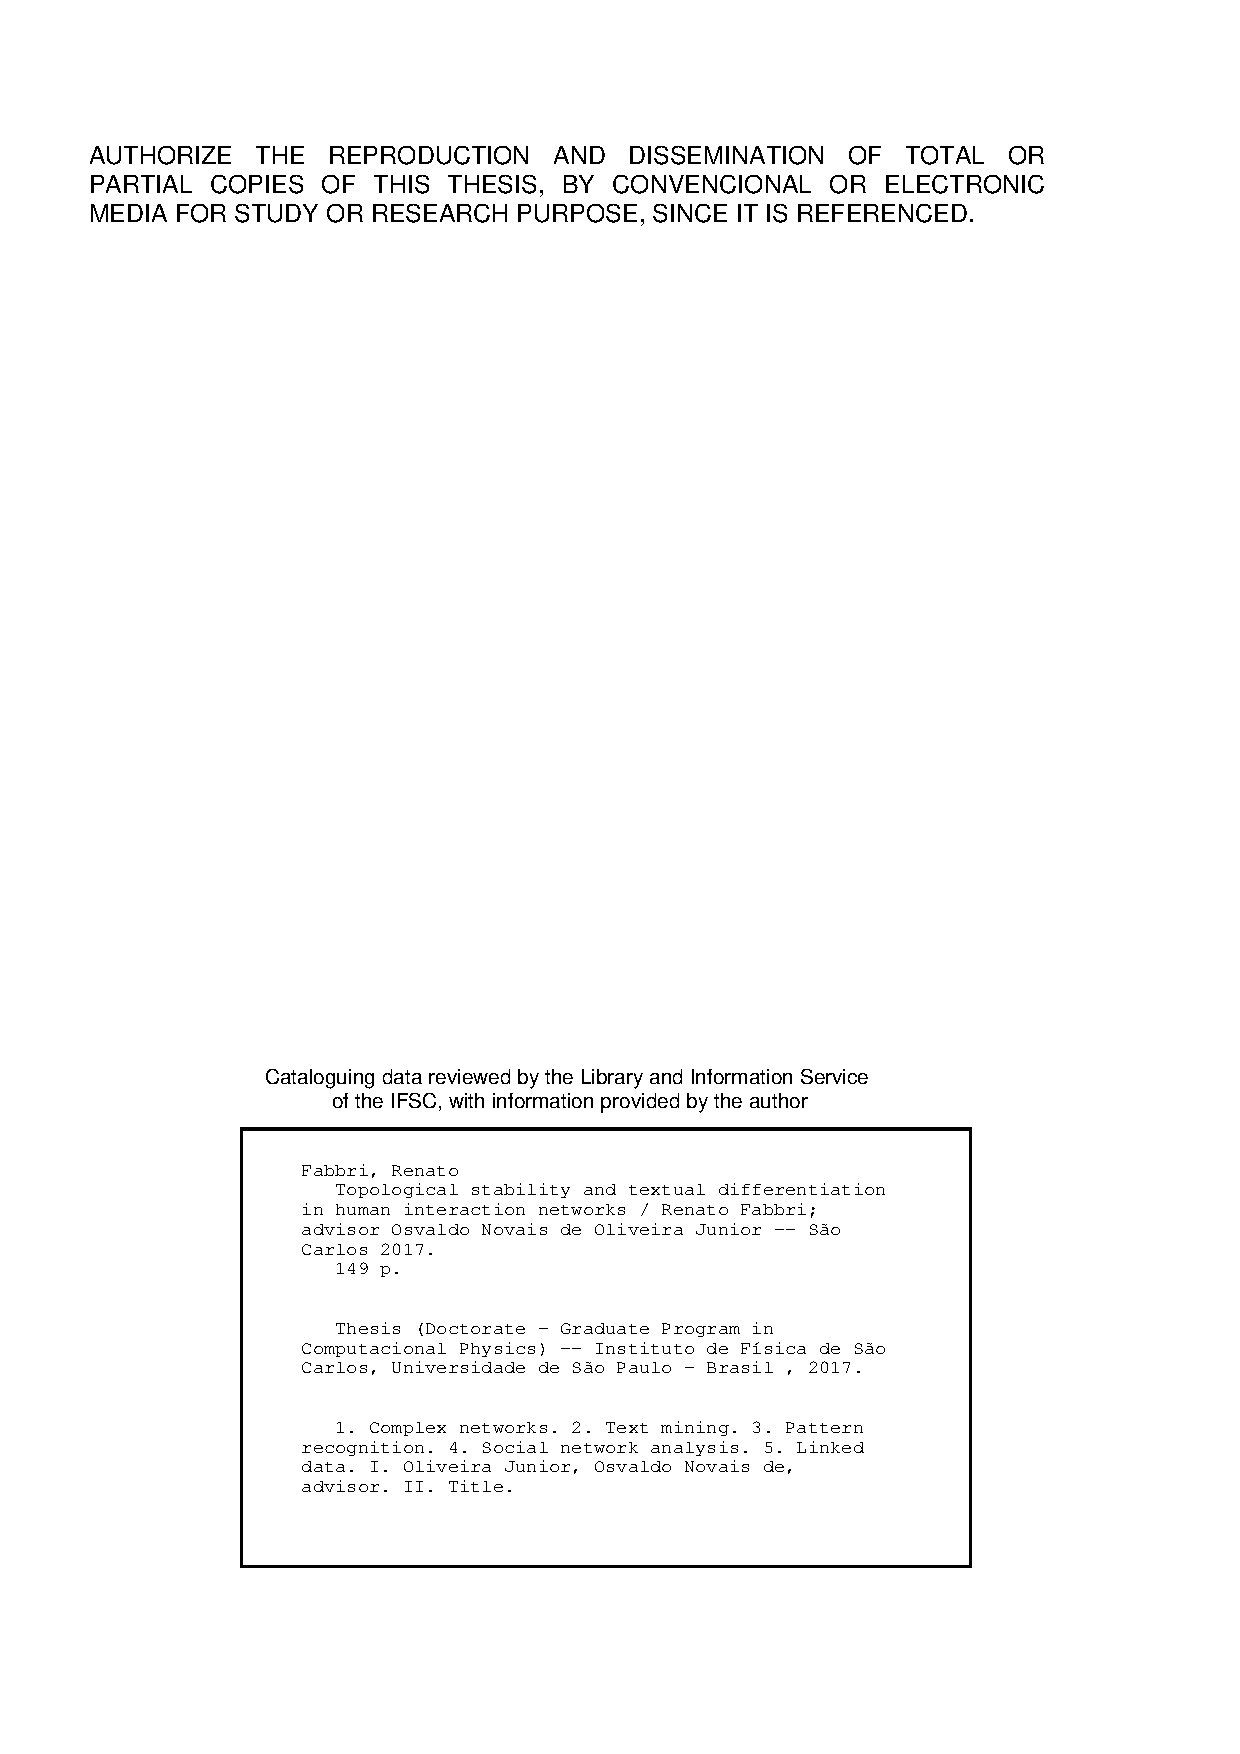
\includepdf{fichacatalografica.pdf}
\end{fichacatalografica}
% Se você optar por elaborar a ficha catalográfica, deverá 
% incluir uma % antes das 3 linhas acima e tirar a % antes
% do comando % ---
% Inserir a ficha bibliografica
% ---
% Isto é um exemplo de Ficha Catalográfica, ou ``Dados internacionais de
% catalogação-na-publicação''. Você pode utilizar este modelo como referência. 
% Porém, provavelmente a biblioteca da sua universidade lhe fornecerá um PDF
% com a ficha catalográfica definitiva após a defesa do trabalho. Quando estiver
% com o documento, salve-o como PDF no diretório do seu projeto e substitua todo
% o conteúdo de implementação deste arquivo pelo comando abaixo:
%
\begin{fichacatalografica}
	\hspace{-1.4cm}
	\imprimirnotaautorizacao \\ \\
	%\sffamily
	\vspace*{\fill}					% Posição vertical
	\begin{center}					% Minipage Centralizado
		\imprimirnotabib \\
\begin{table}[htb]
	\scriptsize
	\centering	
	\begin{tabular}{|p{0.9cm} p{8.7cm}|}
		\hline
	      & \\
		  &	  \imprimirautorficha     \\
		
		 \imprimircutter & 
							\hspace{0.4cm}\imprimirtitulo~  / ~\imprimirautor~ ;  ~\imprimirorientadorcorpoficha. -- 	\imprimirlocal, \imprimirdata.   \\
		
		  &  % Para incluir nota referente à versão corrigida no corpo da ficha,
			  % incluir % no início da linha acima e tirar a % do início da linha abaixo
			  %	\hspace{0.4cm} \imprimirtitulo~  / ~\imprimirautor~ ; ~\imprimirorientadorcorpoficha~- ~\imprimirnotafolharosto. -- \imprimirlocal, \imprimirdata.  \\
		
			\hspace{0.4cm}\pageref{LastPage} p. : il. (algumas color.) ; 30 cm.\\ 
		  & \\
		  & 
		    \hspace{0.4cm}\imprimirnotaficha ~--~ 
						  \imprimirunidademin, 
						  \imprimiruniversidademin, 
		                  \imprimirdata. \\ 
		  & \\                 
		   % Para incluir nota referente à versão corrigida em notas,
		    % incluir uma % no início da linha acima e	
		    % tirar a % do início da linha abaixo
		    % & \hspace{0.4cm}\imprimirnotafolharosto \\ 
		  & \\ 
		  & \hspace{0.4cm}1. LaTeX. 2. abnTeX. 3. Classe USPSC. 4. Editoração de texto. 5. Normalização da documentação. 6. Tese. 7. Dissertação. 8. Documentos (elaboração). 9. Documentos eletrônicos. I. \imprimirorientadorficha. 
		   II. Título. \\
	
		     %Se houver co-orientador, inclua % antes da linha (antes de II. Título.) 
		     %          e tire a % antes do comando abaixo 
		     %III. Título. \\   
		  \hline
	\end{tabular}
\end{table}
	\end{center}
\end{fichacatalografica}
% ---


%% ---
% Inserir a ficha bibliografica
% ---
% Isto é um exemplo de Ficha Catalográfica, ou ``Dados internacionais de
% catalogação-na-publicação''. Você pode utilizar este modelo como referência. 
% Porém, provavelmente a biblioteca da sua universidade lhe fornecerá um PDF
% com a ficha catalográfica definitiva após a defesa do trabalho. Quando estiver
% com o documento, salve-o como PDF no diretório do seu projeto e substitua todo
% o conteúdo de implementação deste arquivo pelo comando abaixo:
%
\begin{fichacatalografica}
	\hspace{-1.4cm}
	\imprimirnotaautorizacao \\ \\
	%\sffamily
	\vspace*{\fill}					% Posição vertical
	\begin{center}					% Minipage Centralizado
		\imprimirnotabib \\
\begin{table}[htb]
	\scriptsize
	\centering	
	\begin{tabular}{|p{0.9cm} p{8.7cm}|}
		\hline
	      & \\
		  &	  \imprimirautorficha     \\
		
		 \imprimircutter & 
							\hspace{0.4cm}\imprimirtitulo~  / ~\imprimirautor~ ;  ~\imprimirorientadorcorpoficha. -- 	\imprimirlocal, \imprimirdata.   \\
		
		  &  % Para incluir nota referente à versão corrigida no corpo da ficha,
			  % incluir % no início da linha acima e tirar a % do início da linha abaixo
			  %	\hspace{0.4cm} \imprimirtitulo~  / ~\imprimirautor~ ; ~\imprimirorientadorcorpoficha~- ~\imprimirnotafolharosto. -- \imprimirlocal, \imprimirdata.  \\
		
			\hspace{0.4cm}\pageref{LastPage} p. : il. (algumas color.) ; 30 cm.\\ 
		  & \\
		  & 
		    \hspace{0.4cm}\imprimirnotaficha ~--~ 
						  \imprimirunidademin, 
						  \imprimiruniversidademin, 
		                  \imprimirdata. \\ 
		  & \\                 
		   % Para incluir nota referente à versão corrigida em notas,
		    % incluir uma % no início da linha acima e	
		    % tirar a % do início da linha abaixo
		    % & \hspace{0.4cm}\imprimirnotafolharosto \\ 
		  & \\ 
		  & \hspace{0.4cm}1. LaTeX. 2. abnTeX. 3. Classe USPSC. 4. Editoração de texto. 5. Normalização da documentação. 6. Tese. 7. Dissertação. 8. Documentos (elaboração). 9. Documentos eletrônicos. I. \imprimirorientadorficha. 
		   II. Título. \\
	
		     %Se houver co-orientador, inclua % antes da linha (antes de II. Título.) 
		     %          e tire a % antes do comando abaixo 
		     %III. Título. \\   
		  \hline
	\end{tabular}
\end{table}
	\end{center}
\end{fichacatalografica}
% ---


% As informações que compõem a ficha catalográfica estão 
% definidos no arquivo USPSC-pre-textual-UUUU.tex
% ---


% ---
% Inserir errata
% ---

% \begin{errata}
% 	\OnehalfSpacing 			
% 	A errata é um elemento opcional, que consiste de uma lista de erros da obra, precedidos pelas folhas e linhas onde eles ocorrem e seguidos pelas correções correspondentes. Deve ser inserida logo após a folha de rosto e conter a referência do trabalho para facilitar sua identificação, conforme a ABNT NBR 14724. \cite{nbr14724}.
% 	
% 	Modelo de Errata:
% 		
% 	\begin{flushleft} 
% 			\setlength{\absparsep}{0pt} % ajusta o espaçamento da referência	
% 			\SingleSpacing 
% 			\imprimirautorabr~ ~\textbf{\imprimirtitulo}.	\imprimirdata. \pageref{LastPage}p. 
% 			%Substitua p. por f. quando utilizar oneside em \documentclass
% 			%\pageref{LastPage}f.
% 			\imprimirtipotrabalho~-~\imprimirinstituicao, \imprimirlocal, \imprimirdata. 
%  	\end{flushleft}
% \vspace{\onelineskip}
% \OnehalfSpacing 
% \center
% \textbf{ERRATA}
% \vspace{\onelineskip}
% \OnehalfSpacing 
% \begin{table}[htb]
% 	\center
% 	\footnotesize
% 	\begin{tabular}{p{1.4cm} p{1cm} p{3cm} p{3cm} }
% 		\hline
% 		\textbf{Folha} & \textbf{Linha}  & \textbf{Onde se lê}  & \textbf{Leia-se}  \\
% 			\hline
% 			1 & 10 & auto-conclavo & autoconclavo\\
% 		\hline
% 	\end{tabular}
% \end{table}
% 
% 
% \end{errata}
% ---

% ---
% Inserir folha de aprovação
% ---

% A Folha de aprovação é um elemento obrigatório da NBR 4724/2011 (seção 4.2.1.3). 
% Após a defesa/aprovação do trabalho, gere o arquivo folhadeaprovacao.pdf da página assinada pela banca 
% e iclua o arquivo utilizando o comando abaixo:
\includepdf{folhadeaprovacao.pdf}

% Alternativa para a Folha de Aprovação:
% Se for a sua opção elaborar uma folha de aprovação, insira uma % antes do comando acima que inclui o arquivo folhadeaprovacao.pdf,
% tire o % do comando abaixo e altere o arquivo folhadeaprovacao.tex conforme suas necessidades
%\include{folhadeaprovacao}


\includepdf{PaginaEmBranco.pdf}

% ---
% Dedicatória
% ---
\begin{dedicatoria}
   \vspace*{\fill}
   \centering
   \noindent
   \textit{ Este trabalho é dedicado à Deus e à minha família.} \vspace*{\fill}
\end{dedicatoria}
% ---

% ---
% Agradecimentos
% ---=====
\begin{agradecimentos}
	I thank
Prof. Dr. Osvaldo Novais de Oliveira Junior and Prof. Dr. Luciano da Fontoura Costa
whose research inspired this thesis.

I thank the integrants of the São Carlos Physics Institute,
including the instructors, the administration and the secretariat
for the mindfulness and patience whenever I needed to reach them.

I thank the Brazilian Presidency and the United Nations Development Program for
the partnership established with this research in the year of 2014.

I thank the labMacambira.sf.net collective for numerous discussions and guidance
with regards to free and digital culture.

I thank my family for the invaluable support in every step.

I thank the open source and free software communities for sharing their work,
which made possible the developments presented in this document.
% SGPR, PNUD
% labmacambira
% wife and family
% O Grupo desenvolvedor do Pacote USPSC, atualmente composto da Classe USPSC e do  Modelo para teses e dissertações em \LaTeX\ utilizando a classe USPSC, agradece especialmente ao Luis Olmes, doutorando do Instituto de Ciências Matemáticas e de Computação (ICMC) da Universidade de São Paulo (USP), pelas primeiras orientações sobre o \LaTeX\ .
% 
% Agradecemos ao Lauro César Araujo pelo desenvolvimento da classe  \abnTeX, modelos canônicos e tantas outras contribuições que nos permitiu o desenvolvimento da classe USPSC e seus modelos.
% 
% Os nossos agradecimentos aos integrantes do primeiro
% projeto abn\TeX\, Gerald Weber, Miguel Frasson, Leslie H. Watter, Bruno Parente Lima, Flávio de Vasconcellos Corrêa, Otavio Real
% Salvador, Renato Machnievscz, e a todos que contribuíram para que a produção de trabalhos acadêmicos em conformidade com
% as normas ABNT com \LaTeX\ fosse possível.
% 
% Agradecemos ao grupo de usuários
% \emph{latex-br}{\url{http://groups.google.com/group/latex-br}}, aos integrantes do grupo
% \emph{\abnTeX}{\url{http://groups.google.com/group/abntex2}  e \url{http://www.abntex.net.br/}}~que contribuem para a evolução do \abnTeX.
\end{agradecimentos}
% ---

% ---
% Epígrafe
% ---
\begin{epigrafe}
    \vspace*{\fill}
	\begin{flushright}
		\textit{``The heart of the discerning acquires knowledge, \\
		for the ears of the wise seek it out.''\\
		Proverbs 18:15}
	\end{flushright}
\end{epigrafe}
% ---

% ---
% Resumo
% ---
% Se o idioma do texto for em inglês, o abstract deve preceder o resumo
% resumo em português
\setlength{\absparsep}{18pt} % ajusta o espaçamento dos parágrafos do resumo		
\begin{resumo}
	\begin{flushleft} 
			\setlength{\absparsep}{0pt} % ajusta o espaçamento da referência	
			\SingleSpacing 
			\imprimirautorabr~ ~\textbf{\imprimirtitulo}.	\imprimirdata. \pageref{LastPage}p. 
			%Substitua p. por f. quando utilizar oneside em \documentclass
			%\pageref{LastPage}f.
			\imprimirtipotrabalho~-~\imprimirinstituicao, \imprimirlocal, \imprimirdata. 
 	\end{flushleft}
\OnehalfSpacing 			
 O resumo deve ressaltar o  objetivo, o método, os resultados e as conclusões do documento. A ordem e a extensão  destes itens dependem do tipo de resumo (informativo ou indicativo) e do  tratamento que cada item recebe no documento original. O resumo deve ser
 precedido da referência do documento, com exceção do resumo inserido no
 próprio documento. (\ldots)  Salientamos que os Programas de Pós-Graduação de algumas Unidades exigem o titulo da dissertação ou tese em inglês, tornando necessário a inclusão das referências nos resumos e abstracts, o que foi adotado no presente modelo. As palavras-chave devem figurar logo abaixo do  resumo, antecedidas da expressão Palavras-chave:, separadas entre si por  ponto e finalizadas também por ponto.  \cite{nbr6028}.
 

 \textbf{Palavras-chave}: LaTeX. abnTeX. Classe USPSC. Editoração de texto. Normalização da documentação. Tese. Dissertação. Documentos (elaboração). Documentos eletrônicos. 
\end{resumo}

% ---
% Abstract
% ---
\autor{Silva, M. J.}
\begin{resumo}[Abstract]
 \begin{otherlanguage*}{english}
	\begin{flushleft} 
		\setlength{\absparsep}{0pt} % ajusta o espaçamento dos parágrafos do resumo		
 		\SingleSpacing 
 		\imprimirautorabr~ ~\textbf{\imprimirtitleabstract}.	\imprimirdata.  \pageref{LastPage}p. 
		%Substitua p. por f. quando utilizar oneside em \documentclass
		%\pageref{LastPage}f.
		\imprimirtipotrabalho~-~\imprimirinstituicao, \imprimirlocal, 	\imprimirdata. 
 	\end{flushleft}
	\OnehalfSpacing 
   This is the english abstract.

   \vspace{\onelineskip}
 
   \noindent 
   \textbf{Keywords}: LaTeX. abnTeX. USPSC class. Text editoration. Standardization of documentation. Thesis. Dissertation. Documents (development). Electronic documents.
 \end{otherlanguage*}
\end{resumo}

% ---
% inserir lista de ilustrações
% ---
\pdfbookmark[0]{\listfigurename}{lof}
\listoffigures*
\cleardoublepage
% ---

% ---
% inserir lista de tabelas
% ---
\pdfbookmark[0]{\listtablename}{lot}
\listoftables*
\cleardoublepage
% ---

% ---
% inserir lista de quadros
% ---
\pdfbookmark[0]{\listofquadroname}{loq}
\listofquadro*
\cleardoublepage
% ---

% ---
% inserir lista de abreviaturas e siglas
% ---
\begin{siglas}
    \item[ABNT] Associação Brasileira de Normas Técnicas
    \item[abnTeX] ABsurdas Normas para TeX
	\item[EESC] Escola de Engenharia de São Carlos
	\item[IAU] Instituto de Arquitetura e Urbanismo
	\item[IBGE] Instituto Brasileiro de Geografia e Estatística
	\item[ICMC] Instituto de Ciências Matemáticas e de Computação
	\item[IFSC] Instituto de Física de São Carlos
	\item[IQSC] Instituto de Química de São Carlos
	\item[USP] Universidade de São Paulo
	\item[USPSC] Campus USP de São Carlos
	
\end{siglas}
% ---

% ---
% inserir lista de símbolos
% ---
\begin{simbolos}
  \item[$ \Gamma $] Letra grega Gama
  \item[$ \Lambda $] Lambda
  \item[$ \zeta $] Letra grega minúscula zeta
  \item[$ \in $] Pertence
\end{simbolos}
% ---
% ---
% inserir o sumario
% ---
\pdfbookmark[0]{\contentsname}{toc}
\tableofcontents*
\cleardoublepage
% ---
% ----------------------------------------------------------
% ELEMENTOS TEXTUAIS
% ----------------------------------------------------------
\textual
% Os capítulos são inseridos como arquivos externos 

% Capítulo 1 - Introdução
% ---
%% USPSC-Introducao.tex
% ----------------------------------------------------------
% Introdução (exemplo de capítulo sem numeração, mas presente no Sumário)
% ----------------------------------------------------------
% \chapter[Introdução]{Introdução}
\chapter{Introduction}\label{ch:int}
The first studies dealing explicitly with human interaction networks
date from the nineteenth century while the foundation of
social network analysis is generally attributed to the psychiatrist Jacob Moreno in mid twentieth century~\cite{moreno,newmanBook}.
With the increasing availability of data related to human interactions, research about these networks has grown continuously.
Contributions can now be found in a variety of fields, from social sciences and humanities~\cite{latour2013} to computer science~\cite{bird} and physics~\cite{barabasiHumanDyn,newmanFriendship}, given the multidisciplinary nature of the topic.
One of the approaches from an exact science perspective is to represent interaction networks as complex networks~\cite{barabasiHumanDyn,newmanFriendship}, with which 
several features of human interaction have been revealed.
For example, the topology of human interaction networks exhibits a scale-free outline,
which points to the existence of a small number of highly connected hubs and a large number of poorly connected nodes.
The dynamics of complex networks representing human interaction has also been addressed~\cite{barabasiEvo,newmanEvolving}, but only to a limited extent, since research is normally focused on a particular metric or task, such as accessibility or community detection~\cite{access,newmanModularity}. 





There are numerous articles, books, websites and software tools about complex and social networks and about text mining in social media.
There are fewer endeavours to characterize these networks beyond general features such as the scale-free 
aspect or to deal with text produced by social networks from the complex networks background.
Research on network evolution is often restricted to network growth, in which there is a monotonic increase in the number of events~\cite{barabasiEvo}.
Network types have been discussed with regard to the number of participants, intermittence of their activity and network longevity~\cite{barabasiEvo}. Two topologically different networks emerged from human interaction networks, depending on whether the frequency of interactions follows a generalized power law or an exponential connectivity distribution~\cite{barabasiTopologicalEv}. In email list networks, scale-free properties were reported with $\alpha \approx 1.8$~\cite{bird} (as in web browsing and library loans~\cite{barabasiHumanDyn}), and different linguistic traces were related to weak and strong ties~\cite{Gmane2}.

In this thesis, e-mail lists were chosen to represent human interaction networks, which were analyzed according to two broad aspects: the possible stability of the topology of the networks and the linguistic usage of distinct types of participants in the network. In the analysis, the topology of the networks was studied with regard to well-established topological metrics and well-established networks models. The text of the networks was studied with regard to statistics derived from the strings and from syntactics and semantics.
The fact that unreciprocated edges often exceed 50\% in human interaction networks~\cite{newmanEvolving} motivated the inclusion of symmetry metrics in our analysis. 
No correlation of topological characteristics and geographical coordinates was found~\cite{barabasiGeo},
therefore geographical positions were not considered in our study.
Gender related behavior in mobile phone datasets was indeed reported~\cite{barabasiSex}
but it is not relevant for the present work because email messages and addresses have no gender related metadata~\cite{gmanePack}. As for the language usage in the networks, emphasis was given to statistical features of the text such as number of tokens and known words, sizes of tokens, known words, sentences and messages. 
Statistics were also derived from syntactics through POS tags (e.g. nouns, adjectives, verbs) and semantics through Wordnet synsets.

The remainder of this chapter provides some background knowledge relevant to the topics discussed in the thesis, especially complex networks, text mining, graph visualization and linked data. In Chapter 2, the data and methods where described while the results and discussion are in Chapter~\ref{ch:disc}. 
Conclusions and further work are stated in Chapter~\ref{ch:concl}.
The appendices bring further results from this research.


\section{Related knowledge}
\subsection{Complex networks}
Although not universally accepted, it is commonplace to define a complex network to be
a ``graph with non-trivial topological features''~\cite{newmanBook}.
We might add to this definition that a complex network is also a large graph (even though no consensus appears to exist as 
to what \emph{large} means in this context)
and that it is a graph representation of a system found in natural, real or empirical system.
Another way to approach the definition of ``complex networks'' is to define it as
complex systems modeled as networks.
This second definition is also useful but is even more problematic as
there is no consensus of what a \emph{complex system} is.
Even so, one should keep in mind that authors often define a complex system
to be a system composed with many parts in which ``the whole is more than
the sum of its parts''.
Authors also often consider complex systems to have capabilities
to ``process information'', to adapt and to reproduce~\cite{complexity}.

A graph is a structure that consists of a set of objects (called vertices)
and a set of binary/dual relations of the objects (called edges).
A graph might be unweighted and undirected (the simplest possibility),
weighted and undirected, unweighted and directed, or weighted and directed.

The most usual representations of graphs (and networks) are the matrix, list and node-edge representations.
In the matrix representation, each entry $a_{ij}$ is non-zero if $i$ is linked to $j$;
entries might be other than 0 and 1 in weighted graphs; undirected graphs yield symmetric matrices.
There are two common list representations of graphs, one lists each pair of vertices that are connected,
the other holds a list for each vertex in which are all the vertices connected to it (a list of lists).
In the node-edge representation, each node is represented as a point while each edge is represented
by a line between corresponding nodes.
The matrix representation is essential for algebraic reasoning and for deriving metrics
while the node-edge representation is important for illustration and intuitive guidance
in characterizing the systems.

\subsubsection{A good justification for applying the complex networks theory}
The estimated number of atoms in the universe, often used as a reference of largeness,
is $\approx 10^{80}$.
Let us find the number of vertices needed to reach such number of possible networks.
Consider the simplest case of the unweighted and undirected networks.
Each edge can exist or not (i.e. it is a Bernoulli variable) and with $n$ vertices there are
at most ${n \choose 2}$ edges.
Therefore:
\begin{align}
2^{n \choose 2} > 10^{80} \Rightarrow 
log_2[2^{n \choose 2}] > log_2(10^{80}) \Rightarrow
{n \choose 2} > \frac{log_{10}(10^{80})}{log_{10}2} \Rightarrow \nonumber\\
\Rightarrow \frac{n.(n-1)}{2} > \frac{80}{log_{10}2} \Rightarrow
N > 23,5988 \;\;\;\;\;\;\;\;\;\;\;\;\;\;\;\;\;\;\;\;\;
\nonumber
\end{align}
That is, with only 24 vertices we have more possible networks than
the estimated number of atoms in the universe.
We should also add that the number of possible networks grows
very fast with the number of vertices.
This is a good reason for characterizing such systems by means
of paradigmatic networks and generic metrics for nodes and the network (and edges, but it is less often).

\subsubsection{Basic metrics}\label{se:intMea}
Section~\ref{measures} gives a mathematical account of the following metrics,
which are used here for characterizing basic types
of networks in the next section.
Such metrics are:
\begin{itemize}
\item Degree $k_i$: number of edges linked to vertex $i$.
\item In-degree $k_i^{in}$: number of edges ending at vertex $i$.
\item Out-degree $k_i^{out}$: number of edges departing from vertex $i$.
\item Strength $s_i$: sum of weights of all edges linked to vertex $i$.
\item In-strength $s_i^{in}$: sum of weights of all edges ending at vertex $i$.
\item Out-strength $s_i^{out}$: sum of weights of all edges departing from vertex $i$.
\item Betweenness centrality $bt_i$: fraction of geodesics that contain vertex $i$.
\item Clustering coefficient $cc_i$: fraction of pairs of neighbors of $i$ that are linked, i.e. the standard clustering coefficient metric for undirected graphs.
\end{itemize}
% distance between vertices
In the following discussion, we also use the concept of distance between a pair of nodes,
which is the number of edges between the nodes.

\subsubsection{Basic types of networks}
Complex networks are often characterized in terms of paradigmatic models.
There are diverse models, but we can glimpse the background theory
with the following ones~\cite{luMeasures}:
\begin{itemize}
\item The Erdös-Rényi model\footnote{This name is also used for the model in which, for a fixed number of nodes and a fixed number of links, all networks are equally likely. This is the model originally introduced by Paul Erdös and Alfréd Rényi~\cite{erdosOrig}.
We choose the definition given in the main text, which is closely related to the one given in this footnote, because it is more commonly used nowadays.}: each pair of nodes is connected with a fixed random probability $p$.
This model presents a characteristic degree ($n.p$ where $n$ is the number of nodes), low clustering and low average distance between nodes.
\item Spatial network, also called geographic network or geometric graph: nodes are located in a metric space and the probability that two nodes are connected is greater as the distance between nodes gets smaller. These networks present characteristic degrees, high clustering and large average distance between nodes.
\item Small-word network: defined as a network where the typical distance between nodes grows with the logarithm of the number of nodes while the average clustering coefficient is not small (larger than e.g. in the Erdös-Rényi model).
One method for constructing a small-world network is to start with a regular lattice in which each node is connected to $k$ nearest neighbors.
Each link is then rewired with probability $p$.
With intermediate values of $p$ such as $0.01<p<0.1$, we obtain a network with both short average distance between nodes (as in the Erdös-Rényi model) and a high average clustering coefficient (as in the spatial network).
This model presents a characteristic degree.
\item Scale-free networks: in which the degree distribution $p(k)$ follows a power law ($p(k)=C.k^{-\alpha}$ where $C$ and $\alpha$ are constants).
These networks are qualitatively characterized by the presence of a large number of poorly connected and of few highly connected hubs.
Important is the absence of a characteristic degree, thus the name 'scale-free network'.
\item Other networks: among important models of networks are exponential networks, networks with community structure and hybrid models.
\end{itemize}
Real networks most often exhibit scale-free and small-world properties.
This is the case of most e.g. social, gene and food networks.
However, one should be cautious about such statement because
the networks derived from the real systems depend heavily
in what is considered a node and a link,
i.e. on how the system is modeled as a graph.
Another noteworthy remark is that
the Erdös-Rényi networks, i.e. graphs of the Erdös-Rényi model, are frequently pin-pointed as the networks with trivial
topological properties.
This model is considered as a paradigmatic ``complex network'', concept often defined as graphs with non-trivial topological properties,
which is a contradiction. Therefore, the term complex networks is not a very well defined notion, as it occurs for the \emph{complexity theory} in general.


\subsection{Text mining of social data}
Text mining is a multidisciplinary field,
it is an extension of data mining to (often unstructured) textual data
with the goal of discovering structure and meaning~\cite{customText}.
A general outline of a text mining endeavor involves structuring input text,
deriving patterns and the evaluation of the output.
There are actually numerous models of such outline,
as e.g. considering document collection and obtaining a final report in the
start and end respectively~\cite{textSurvey}.
Text mining tasks include document summarization, sentiment analysis
and natural language processing techniques such as part of speech tagging~\cite{ntlk}.
Among the applications one may include social media monitoring, automated ad placement, and development of tools for 
semantics ~\cite{textSurvey}.
It is believed that applying text mining to social media
can yield interesting findings in human behavior~\cite{customText}.
Although there is no clear cut, text mining is sometimes divided into linguistic and non-linguistic~\cite{customText}.
In the first case, techniques borrowed from linguistics are present, such as
the analysis of discourse and part of speech tagging,
and it is often mingled with natural language processing or computational linguistics (see Section~\ref{amb} for a coherent distinction of the fields).
In the non-linguistic text mining, text is analyzed by means of statistical features
derived from e.g. the size of tokens and sentences,
and might be more easily related to the intuitive concept of data mining of text.
In this thesis we use both perspectives.

\subsection{Visualization of static and dynamic graphs}
Static graph visualization is achieved in many ways,
most usually through the node-link (often called network diagram)
and matrix representations.
Representing graphs as node-link diagrams has a long tradition which goes back 
at least to the works of Ramon Llull in the 13th century~\cite{llull}.
To glimpse at the theory involved in visualizing networks~\cite{eades}, we mention three aspects:
\begin{itemize}
\item criteria for the quality of layouts might include the number of crossing edges or the area of the drawing relative to the closest distance between two vertices.
\item Layout methods are derived e.g. by placing vertices in a circular fashion, by using the eigen vectors from a worked out variant of the adjacency matrix as coordinates, or by force-based methods. For large graphs, including a number of social networks, the force-based networks are reported as useful. Therefore, we illustrate this method with the simplest model we could find in the specialized literature. Let $f_a$ be the attraction force, $f_r$ is the repulsion force, $d$ is the distance between the vertices and $k$ is a constant. The model introduced by Fruchterman and Reingold~\cite{fr} defines the forces as:
\begin{align}
f_a = \frac{d^2}{k}\\
f_d = -\frac{k^2}{d}
\end{align}
On a computer software, one usually starts with a random layout and performs a number of iterations updating the position of nodes
using these forces to obtain the intended force-directed layout.
\item Graph drawings are often developed for specific applications e.g. in biology (as for protein and gene interactions), in social networks, in tree diagrams.
\end{itemize}

The core difference of dynamic graphs to static graphs is that vertices and edges
can be added and removed over time.
If we define the static graph G as $G:=(V,E)$ where V are the vertices as E are the edges in G,
a dynamic graph might be defined as $\Gamma:=(G_1,G_2,...,G_n)$ where $G_i:=(V_i,E_i)$
are static graphs and indices refer to a sequence of time steps $(t_1,t_2,...,t_n)$.
In dynamic graph visualization most usually graphs are represented as animated diagrams
or charts based on a timeline~\cite{dynGraph}.
In this thesis we make use of node-link diagrams of both static and dynamic graphs.

\subsection{Linked (open) data}
The fields of social network analysis and complex networks
are widely researched.
However, there is a lack of open datasets for benchmarking results,
especially associated with the complex networks field,
yielding diverse results from poorly related sources.
Recently, a myriad of results have been reported which are based on
diverse datasets most often not accessible to researchers other than the publishing authors.
In this thesis we present resources for having open databases to provide 
the scientific community with a friendly and common repertoire.
We chose to use the linked data technology and follow W3C best practices for publishing data.

Linked data refers to data published in the web in such a way that it is
machine readable and complies with a set of best practices.
The web of data is constructed with documents on the web 
such as the web of HTML documents.
In practice, the idea of linked data can me summarized
by 1) the use of RDF to publish data on the web and 2) the use of RDF
links to interlink data from different sources.
The web is expected to be interconnected and to grow by the systematic application of four
steps~\cite{lee1}:
\begin{itemize}
\item Use URIs to identify things~\cite{uri}.
\item Use HTTP URIs.
\item Provide useful information when an URI is accessed via HTTP.
\item Provide other URIs in the description of resources so human
and machine agents can perform discovery.
\end{itemize}

The Linked Open Data~\cite{lod} builds an ever growing cloud of data,
the global data space, which is usually
conceived as centered around the DBPedia, a linked data representation
of data from Wikipedia~\cite{dbpedia0,dbpedia}.

\subsubsection{RDF}
The Resource Description Framework (RDF), a W3C
recommendation, is a model for data
interchange.
It is based on the idea of making statements about resources in the form
of triples, i.e. expressions in the form ``subject - predicate -
object''.
RDF can be serialized in several file formats, including RDF/XML,
Turtle and Manchester, all of which, in essence, represent a labeled and
directed multi-graph.
RDF may be stored in a type of database referred to as a triplestore~\cite{rdf}.

As an example of an RDF statement, the following triple in the Turtle
format asserts that ``the paper has color white'':\\
\texttt{http://example.org/Things\#Paper http://example.org/hasColor\\
http://example.org/Colors\#White .}
% This work makes available an open database with diverse provenance and
% to furnish the scientific community with a friendly and common repertoire.

Integration and uniformity of access is obtained through linked data
representation, as explained in Section~\ref{queries}.

\subsection{Social participation}
A significant share of our endeavor was oriented towards social participation,
i.e. to facilitate civil engagement in a community, most significantly in State affairs.
More concretely, we published data from a social participation federal portal~\cite{losd},
applied complex networks and text mining criteria for resources recommendation~\cite{pnud3,pnud4,opa} and
proposed a ranking algorithm for voted proposals in another federal participation portal~\cite{dialogaAlg}.
Such works were performed within a United Nations Development Program consulting contract,
in partnership with the Brazilian Presidency of the Republic and published publicly mainly as technical reports~\cite{pnud3,pnud4,opa}.
This aspect of our research was important for maturing topics and understanding
the extent to which they are applied in pragmatic contexts.
It is left mostly as subsidiary documents in this thesis to allow for an easy public access.

\subsection{Other}
Given the multidisciplinary condition of our work and of the implied topics,
many other fields of knowledge could be further explored in this introduction or
the methods chapter.
To name just a few of the most directly related fields: statistics, principal component analysis,
big data, social network analysis, social media mining, mathematical sociology,
datasets, free culture, open source software, computer programming.

Of particular relevance are the typologies for human personality, such as the ones derived
from the Myers-Briggs type indicator~\cite{mb} and from authoritarian personality~\cite{adorno} theories,
because we present a new typology of human participants in social networks in Section~\ref{sec:pty}.
Another topic we should highlight is what we called ``anthropological physics''~\cite{anPhy,antphy2}:
the observation of natural/physical laws in human social systems.
The term should not be confused with physical anthropology, which is a synonym for biological anthropology,
a subfield of anthropology concerned with the evolution of humans~\cite{phyAn}.

\section{Polysemy and synonyms}\label{amb}
In the context of complex networks, the words \emph{network} and \emph{graph}
are often used interchangeably, although the word graph might refer to the
mathematical structure of vertices and edges and the word network might refer to the
real system being represented as a graph or to the graph obtained by means of representing a real system.
Furthermore, the word graph can be used to refer to a \emph{graph of a function} (mathematics) or to an abstract datatype (computer science).
This parallelism between network and graphs also apply to network visualization and graph visualization.
One might add here the term \emph{graph drawing}, another synonym for the visualization of graphs, although the term
seems to be more traditional in relation to the achievement of node-edge network diagrams.
Evolutionary graph visualization or evolutionary network visualization are examples of variants of \emph{dynamic graph visualization}.
The nomenclature of vertices and edges varies widely among interested fields (mathematics, physics, biology, sociology, etc).
A vertex might be called e.g. a node, a point, an agent, an actor, a participant.
An edge might be called e.g. a link, a bond, a relation, a tie, a connection.

% There is also some ambiguity related to metrics that can be take with respect to each vertex (or, less often, to each edge),
% such as degree and clustering.
% Such terms might be also used for the average of the measure for the whole network.

The terms \emph{text mining}, \emph{natural language processing} and \emph{computational linguistics}
are often used for similar endeavors.
A distinction might be made in that text mining refers to data mining of text,
natural language processing is concerned with the interactions between the computer and the human natural languages,
and computational linguistics aims for statistical or rule-based modeling of natural language from a computational perspective.
Such fields are multidisciplinary and there is no sharp distinction between them.

Examined as fields of knowledge, the \emph{linked data} and the \emph{semantic web}
terms are often used without distinction.
Tim Berners-Lee coined both terms: 
the semantic web was conceived as a web of data that can be processed by machines~\cite{lee0},
the expression linked data appeared in a 2006 design note about the Semantic Web project~\cite{lee1}
and refers to structured data that emphasizes interlinking and usefulness through semantic queries.

\emph{Social participation}, \emph{social involvement} and \emph{social engagement} are synonyms that
refer to the participation of an individual or group in a community or society.
In Brazilian Portuguese, \emph{controle social} can refer to the antagonist concepts of social participation
or of a social control (played by the State or companies in the civil society).

\subsection{More specific terminology problems in the complex networks field}
Given that this thesis involves multidisciplinary and new knowledge,
it might be of no surprise that the nomenclature is not very well defined.
Here we pin-point some more specific conflicts that arise in the literature of complex networks
to both exemplify this issue and to avoid some problems in interpreting the
methods and results in this thesis:


\begin{itemize}
\item The \emph{hubs} are, by the usual definition, the more connected vertices.
In the context of the HITS (Hyperlink-Induced Topic Search) algorithm,
for attributing centrality to vertices, most traditionally to web pages,
the hubs are the vertices with greater out-degree
(greater in-degree yield \emph{authorities}).
\item In some contexts, the center of network is the collection of vertices whose 
maximum distance to other vertices is the radius (i.e. the minimum maximum difference between vertices). 
In the same framework, the periphery of a network is the collection of vertices whose
maximum distance to other vertices is the diameter (i.e. the maximum distance between vertices).
By extension, the intermediary might be regarded as the set of vertices that are not in the center or the periphery.
These definitions yield fractions of members that do not agree with the literature with respect to hubs, intermediary and periphery.
We present a suitable method for deriving such classification, in the sense that it fits the literature prediction, in Section~\ref{sectioning}.
\item Lace, loop, selfloop and autoloop are terms used to designate an edge from a vertex to itself.
\end{itemize}

\section{Historical note}
The knowledge fields involved in this thesis are very recent.
To point just the main areas,
complex networks has emerged in the final years of the 1990s decade~\cite{newmanBook};
text mining first workshops were held in 1999~\cite{textMining};
as an independent field, graph drawing arose in the 1990s~\cite{dynGraph};
the term linked data was coined in 2006~\cite{lee1}.
% fields are recent, point starting works and/or dates for the fields.

\section{Further considerations}
An initial proposal of this research was to enable
the use of complex and social networks scientific knowledge by the participant of the networks.
This motivated the open software, data and texts produced, conferences attended, and the endeavors with
the United Nations, Brazilian Presidency and civil parties.
As this was a practical goal, we found by hands-on processes that
many fields are deeply related to the subject, which reflected in the number of fields tackled in this thesis
and related documents~\cite{pnud3,pnud4,opa,anPhy,antphy2,dialogaAlg,losd,versinus,kolmSmir}.
Furthermore, we understand that the open software, texts, videos and processes provided
by our work contributes for the popularization of the knowledge and technologies implied
by the empowerment of civil individuals and groups through the management of the
networks in which they exist.

% canonical chapters; stability through circular statistics and topological statistics (PCA, sectioning)
% text mining through measures of sizes of tokens, sentences, messages
% through kolmogorov-smirnov, POS tagging, PCA
% visualization of network evolution through animations (and other gadgets)
% linked data representation of data and ontological organization
% Appendices: supporting tables and diagrams, related results:

% kolmogorov-smirnov, ubiquity of inequality through power laws, list of UNDP products, list of software

% ---

% ---
% Capítulo 2
% ---
\include{USPSC-Cap2-Desenvolvimento}
% ---
% Capítulo 3 - Citações
% ---
\include{USPSC-Cap3-Citacoes}

% ---
% Capítulo 4 - Referencias
% ---
\include{USPSC-Cap4-Referencias}
% ---

% Capítulo 5 - Conclusão
% ---
\include{USPSC-Cap5-Conclusao}
% ---

% ----------------------------------------------------------
% ELEMENTOS PÓS-TEXTUAIS
% ----------------------------------------------------------
\postextual
% ----------------------------------------------------------

% -----------------------------------------------------------
% Referências bibliográficas
% ----------------------------------------------------------
\bibliography{USPSC-modelo-references}


% ----------------------------------------------------------
% Glossário
% ----------------------------------------------------------
%
% Consulte o manual da classe abntex2 para orientações sobre o glossário.
%
%\glossary

% ----------------------------------------------------------
% Apêndices
% ----------------------------------------------------------
%% USPSC-Apendice.tex
% ---
% Inicia os apêndices
% ---

\begin{apendicesenv}
	% Imprime uma página indicando o início dos apêndices
	\partapendices
	\chapter{Additional tables of the textual differences found in all networks}\label{ap:textd}
In the following tables the counting of differences of textual features among the analyzed networks
are shown.
	These results are auxiliary for the discussion on Section~\ref{sec:tresults}.
\FloatBarrier
\begin{table}[h!]
\begin{center}
\caption{Counts of evidence of characters-related differences in the Erd\"os sectors in each of the analyzed networks.}
	\def\arraystretch{1.5}
\begin{tabular}{| l || c | c | c || c |}\hline
{\bf synset} & {\bf p.} & {\bf i.} & {\bf h} & {\bf peaks} \\\hline\hline
$\frac{spaces}{chars}$ & 2  & 0  & 8  & 2 \\
$\frac{punct}{chars-spaces}$ & 11  & 4  & 1  & 5 \\
$\frac{digits}{chars-spaces}$ & 9  & 7  & 2  & 10 \\\hline
$\frac{letters}{chars-spaces}$ & 0  & 0  & 3  & 0 \\
$\frac{vowels}{letters}$ & 0  & 1  & 1  & 1 \\
$\frac{uppercase}{letters}$ & 13  & 3  & 1  & 6 \\\hline
\end{tabular}
\begin{flushleft}
		Source: By the author.\
\end{flushleft}
\end{center}
\end{table}

\begin{table}[h!]
\begin{center}
\caption{Counts of evidence of token-related differences in the Erd\"os sectors in each of the analyzed networks.}
	\def\arraystretch{1.5}
\begin{tabular}{| l || c | c | c || c |}\hline
{\bf synset} & {\bf p.} & {\bf i.} & {\bf h} & {\bf peaks} \\\hline\hline
$\frac{knownw}{tokens}$ & 1  & 0  & 5  & 1 \\
$\frac{knownw \neq}{knownw}$ & 13  & 1  & 4  & 9 \\
$\frac{stopw}{knownw}$ & 0  & 0  & 14  & 2 \\
$\frac{punct}{tokens}$ & 10  & 3  & 1  & 3 \\
$\frac{contrac}{tokens}$ & 0  & 2  & 15  & 4 \\\hline
$\mu(\overline{tokens})$ & 0  & 1  & 2  & 1 \\
$\sigma(\overline{tokens})$ & 7  & 1  & 0  & 2 \\\hline
$\mu(\overline{knownw})$ & 0  & 0  & 2  & 0 \\
$\sigma(\overline{knownw})$ & 0  & 0  & 1  & 1 \\\hline
$\mu(\overline{knownw \neq})$ & 0  & 0  & 0  & 0 \\
$\sigma(\overline{knownw \neq})$ & 0  & 0  & 0  & 0 \\\hline
$\mu(\overline{stopw})$ & 0  & 0  & 0  & 0 \\
$\sigma(\overline{stopw})$ & 0  & 0  & 1  & 0 \\\hline
\end{tabular}
\begin{flushleft}
		Source: By the author.\
\end{flushleft}
\end{center}
\end{table}

\begin{table}[h!]
\begin{center}
\caption{Counts of evidence of sentence-related differences in the Erd\"os sectors in each of the analyzed networks.}
\begin{tabular}{| l || c | c | c || c |}\hline
{\bf synset} & {\bf p.} & {\bf i.} & {\bf h} & {\bf peaks} \\\hline\hline
$\mu_S(chars)$ & 9  & 3  & 1  & 6 \\
$\sigma_S(chars)$ & 11  & 6  & 1  & 9 \\\hline
$\mu_S(tokens)$ & 10  & 2  & 1  & 5 \\
$\sigma_S(tokens)$ & 9  & 7  & 1  & 9 \\\hline
$\mu_S(knownw)$ & 9  & 3  & 2  & 6 \\
$\sigma_S(knownw)$ & 11  & 5  & 2  & 8 \\\hline
$\mu_S(stopw)$ & 2  & 3  & 7  & 7 \\
$\sigma_S(stopw)$ & 6  & 7  & 4  & 10 \\\hline
$\mu_S(puncts)$ & 13  & 2  & 1  & 2 \\
$\sigma_S(puncts)$ & 7  & 8  & 1  & 8 \\\hline
\end{tabular}
\begin{flushleft}
		Source: Prepared by the authors.\
\end{flushleft}
\end{center}
\end{table}

\begin{table}[h!]
\begin{center}
\caption{Counts of evidence of message-related differences in the Erd\"os sectors in each of the analyzed networks.}
	\def\arraystretch{1.5}
\begin{tabular}{| l || c | c | c || c | c |}\hline
{\bf synset} & {\bf p.} & {\bf i.} & {\bf h} & {\bf peaks} & {\bf total} \\\hline\hline
$\mu_M(sents)$ & 4  & 7  & 1  & 9  & 16 \\
$\sigma_M(sents)$ & 5  & 7  & 2  & 11  & 15 \\\hline
$\mu_M(tokens)$ & 10  & 5  & 2  & 6  & 18 \\
$\sigma_M(tokens)$ & 8  & 8  & 2  & 9  & 18 \\\hline
$\mu_M(knownw)$ & 8  & 5  & 3  & 7  & 18 \\
$\sigma_M(knownw)$ & 10  & 5  & 3  & 9  & 18 \\\hline
$\mu_M(stopw)$ & 5  & 6  & 6  & 8  & 18 \\
$\sigma_M(stopw)$ & 7  & 6  & 3  & 11  & 18 \\\hline
$\mu_M(puncts)$ & 12  & 4  & 2  & 5  & 18 \\
$\sigma_M(puncts)$ & 8  & 9  & 1  & 10  & 18 \\\hline
$\mu_M(chars)$ & 10  & 5  & 2  & 6  & 18 \\
$\sigma_M(chars)$ & 9  & 7  & 2  & 8  & 18 \\\hline
\end{tabular}
\begin{flushleft}
		Source: Prepared by the authors.\
\end{flushleft}
\end{center}
\end{table}

\begin{table}[h!]
\begin{center}
\caption{Counts of evidence of differences related to POS tags in the Erd\"os sectors in each of the analyzed networks.}
\begin{tabular}{| l || c | c | c || c |}\hline
{\bf synset} & {\bf p.} & {\bf i.} & {\bf h} & {\bf peaks} \\\hline\hline
NOUN & 13  & 1  & 0  & 1 \\
X & 4  & 9  & 5  & 14 \\\hline
ADP & 0  & 1  & 4  & 1 \\
DET & 1  & 0  & 9  & 2 \\\hline
VERB & 0  & 0  & 6  & 1 \\\hline
ADJ & 1  & 2  & 6  & 2 \\
ADV & 0  & 0  & 17  & 1 \\\hline
PRT & 1  & 1  & 9  & 4 \\
PRON & 0  & 1  & 11  & 3 \\
NUM & 8  & 5  & 3  & 7 \\
CONJ & 2  & 6  & 4  & 8 \\\hline
\end{tabular}
\begin{flushleft}
		Source: By the author.\
\end{flushleft}
\end{center}
\end{table}

\begin{table}[h!]
\begin{center}
\caption{Counts of evidence of differences related to Wordnet POS tags in the Erd\"os sectors in each of the analyzed networks.}
\begin{tabular}{l || c | c | c || c}\hline
{\bf synset} & {\bf p.} & {\bf i.} & {\bf h} & {\bf peaks} \\\hline\hline
N & 8  & 1  & 0  & 1 \\
ADJ & 0  & 2  & 12  & 6 \\
VERB & 0  & 1  & 16  & 2 \\
ADV & 0  & 0  & 9  & 1 \\\hline\hline
POS & 0  & 0  & 3  & 1 \\
POS! & 0  & 1  & 0  & 1 \\\hline
\end{tabular}
\begin{flushleft}\footnotesize
		Source: By the author.\
\end{flushleft}
\end{center}
\end{table}

\begin{table}[h!]
\begin{center}
\caption{Counts of evidence of differences related to Wordnet noun synset characteristics in the Erd\"os sectors in each of the analyzed networks.}
\begin{tabular}{| l || c | c | c || c |}\hline
{\bf synset} & {\bf p.} & {\bf i.} & {\bf h} & {\bf peaks} \\\hline\hline
$\mu(min\,depth)$ & 0  & 0  & 0  & 0 \\
$\sigma(min\,depth)$ & 1  & 1  & 2  & 1 \\\hline
$\mu(max\,depth)$ & 0  & 0  & 0  & 0 \\
$\sigma(max\,depth)$ & 0  & 1  & 3  & 1 \\\hline
$\mu(holonyms)$ & 7  & 4  & 4  & 6 \\
$\sigma(holonyms)$ & 3  & 4  & 7  & 6 \\\hline
$\mu(meronyms)$ & 8  & 5  & 3  & 7 \\
$\sigma(meronyms)$ & 12  & 4  & 2  & 9 \\\hline
$\mu(domains)$ & 6  & 4  & 5  & 8 \\
$\sigma(domains)$ & 3  & 1  & 4  & 3 \\\hline
$\mu(lemmas)$ & 6  & 0  & 1  & 2 \\
$\sigma(lemmas)$ & 6  & 2  & 2  & 4 \\\hline
$\mu(hyponyms)$ & 1  & 6  & 6  & 9 \\
$\sigma(hyponyms)$ & 4  & 6  & 6  & 11 \\\hline
$\mu(hypernyms)$ & 0  & 0  & 0  & 0 \\
$\sigma(hypernyms)$ & 4  & 4  & 4  & 6 \\\hline
\end{tabular}
\begin{flushleft}
		Source: Prepared by the authors.\
\end{flushleft}
\end{center}
\end{table}

\begin{table}[h!]
\begin{center}
\caption{Counts of evidence of differences related to Wordnet adjective synset characteristics in the Erd\"os sectors in each of the analyzed networks.}
\begin{tabular}{| l || c | c | c || c |}\hline
{\bf synset} & {\bf p.} & {\bf i.} & {\bf h} & {\bf peaks} \\\hline\hline
$\mu(domains)$ & 2  & 6  & 8  & 10 \\
$\sigma(domains)$ & 2  & 4  & 5  & 7 \\\hline
$\mu(similar)$ & 1  & 0  & 7  & 4 \\
$\sigma(similar)$ & 4  & 0  & 5  & 3 \\\hline
$\mu(lemmas)$ & 1  & 2  & 1  & 2 \\
$\sigma(lemmas)$ & 6  & 3  & 4  & 6 \\\hline
\end{tabular}
\begin{flushleft}
		Source: By the author.\
\end{flushleft}
\end{center}
\end{table}

\begin{table}[h!]
\begin{center}
\caption{Counts of evidence of differences related to Wordnet verb synset characteristics in the Erd\"os sectors in each of the analyzed networks.}
\begin{tabular}{| l || c | c | c || c |}\hline
{\bf synset} & {\bf p.} & {\bf i.} & {\bf h} & {\bf peaks} \\\hline\hline
$\mu(min\,depth)$ & 2  & 1  & 1  & 3 \\
$\sigma(min\,depth)$ & 2  & 1  & 1  & 2 \\\hline
$\mu(max\,depth)$ & 2  & 1  & 0  & 1 \\
$\sigma(max\,depth)$ & 3  & 1  & 1  & 2 \\\hline
$\mu(domains)$ & 7  & 3  & 4  & 4 \\
$\sigma(domains)$ & 8  & 3  & 3  & 5 \\\hline
$\mu(verb\,groups)$ & 0  & 2  & 3  & 2 \\
$\sigma(verb\,groups)$ & 0  & 0  & 0  & 0 \\\hline
$\mu(lemmas)$ & 0  & 0  & 2  & 0 \\
$\sigma(lemmas)$ & 1  & 0  & 3  & 0 \\\hline
$\mu(entailments)$ & 7  & 1  & 7  & 3 \\
$\sigma(entailments)$ & 4  & 1  & 5  & 3 \\\hline
$\mu(hyponyms)$ & 1  & 2  & 6  & 3 \\
$\sigma(hyponyms)$ & 2  & 3  & 8  & 6 \\\hline
$\mu(hypernyms)$ & 2  & 2  & 0  & 2 \\
$\sigma(hypernyms)$ & 1  & 0  & 1  & 1 \\\hline
\end{tabular}
\begin{flushleft}
		Source: By the author.\
\end{flushleft}
\end{center}
\end{table}

\begin{table}[h!]
\begin{center}
\caption{Counts of evidence of differences related to Wordnet adverb synset characteristics in the Erd\"os sectors in each of the analyzed networks.}
\begin{tabular}{| l || c | c | c || c |}\hline
{\bf synset} & {\bf p.} & {\bf i.} & {\bf h} & {\bf peaks} \\\hline\hline
$\mu(domains)$ & 3  & 3  & 10  & 10 \\
$\sigma(domains)$ & 1  & 4  & 7  & 7 \\\hline
$\mu(lemmas)$ & 0  & 0  & 1  & 1 \\
$\sigma(lemmas)$ & 3  & 1  & 2  & 4 \\\hline
\end{tabular}
\begin{flushleft}
		Source: Prepared by the authors.\
\end{flushleft}
\end{center}
\end{table}


\chapter{Developments made in this research but not included elsewhere in this thesis}\label{ap:vot}
In this appendix are gathered developments relevant for the initial proposal of this research:
enabling the use of complex networks scientific knowledge by the participant of the social networks.
These developments are not included elsewhere in the thesis because we chose to present results
more closely related to physics in a simple fashion.
Furthermore, most of the following contributions have received dedicated documentation,
reason why we next only summarize and cite the documents when they are available.

\section{Continuous voting by approval and participation}
In finding the adequate way to prioritize proposals, the Brazilian social participation community agreed about the measurement of two indexes,
one of approval and one of participation. Both practice and literature
was constantly handled by the experts involved, and the formalization
of such model and metrics and is very simple and seems novel.
Also, the relevance of this development is strengthened by the use of these indexes by the
Brazilian General Secretariat of the Republic to raise and prioritize
proposals about public health care in open processes.
This was achieved by means of the Dialoga Brasil federal platform~\cite{dialoga}.
A short report on these indexes and their use is on~\cite{dialogaAlg}
	(co-authorship by Ricardo Poppi).

	\section{Visualization of static networks}
	In Sections~\ref{sec:versinus0} and~\ref{sec:versinus1} we addressed a visualization method of networks through animations.
	We also made many static network visualizations which were important for our research.
	Many of these were made by testing software and programming libraries.
	We next exemplify such efforts by probably the most important and time-consuming realizations.

	\subsection{Static email networks visualization using Networkx and Graphviz and a PHP web interface}\label{sec:autoRede}
	At the start of this research, we observed many networks derived from email lists
	by means of a web interface we wrote.
	In such web interface, which was accessed as a usual webpage through HTTP in a web browser, 
	the user could specify an email list, start and end messages and a window size (number of messages taken together to obtain the network).
	The interface then rendered graph visualizations and standard measures such as degree, strength, clustering coefficient, betweenness centrality, both as histograms and as mean and standard deviation.
	In the node-link diagrams, measurements were mapped to height, width and color of nodes and to link characteristics.
	The software source code is available in~\cite{autoRede} and an example image is Figure~\ref{fig:autoRede}.
\begin{figure}[h!]
\begin{center}
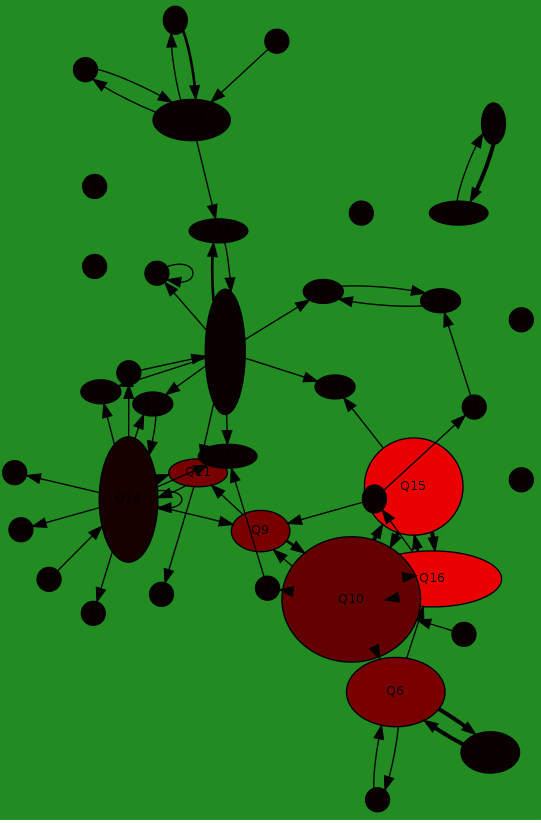
\includegraphics[scale=.25]{figs/autoRede_}
\caption{An example image rendered from the first online gadget made in this research for studying social networks.
	The app also delivered measurements, 2D plots and GML graph files. For further information please see Section~\ref{sec:autoRede}}
\label{fig:autoRede}
\begin{flushleft}\footnotesize
Source: By the author.\
\end{flushleft}
\end{center}
\end{figure}
% email pelo app online

	\subsection{Static Facebook networks visualization using Gephi}\label{sec:gephi}
	Mainly in the years of 2013 and 2014, Facebook users retrieved their friendship networks through Netvizz software~\cite{netvizz}
	and donated them to our research.
	I also retrieved friendship and interaction networks from Facebook groups I was a member, also using Netvizz.
	These networks were used for information collection and diffusion (explained in Section~\ref{sec:colDif}),
	taking measurements and visualization.
	The visualizations were achieved almost exclusively through the Gephi software~\cite{gephi}
	and is included in this appendix for being used a number of times by fellow researchers and artists.
	The most useful layout algorithm was Force Atlas 2~\cite{fa2} and an example of these images is Figure~\ref{fig:gephi}.

% \begin{figure}[h!]
% \begin{center}
% 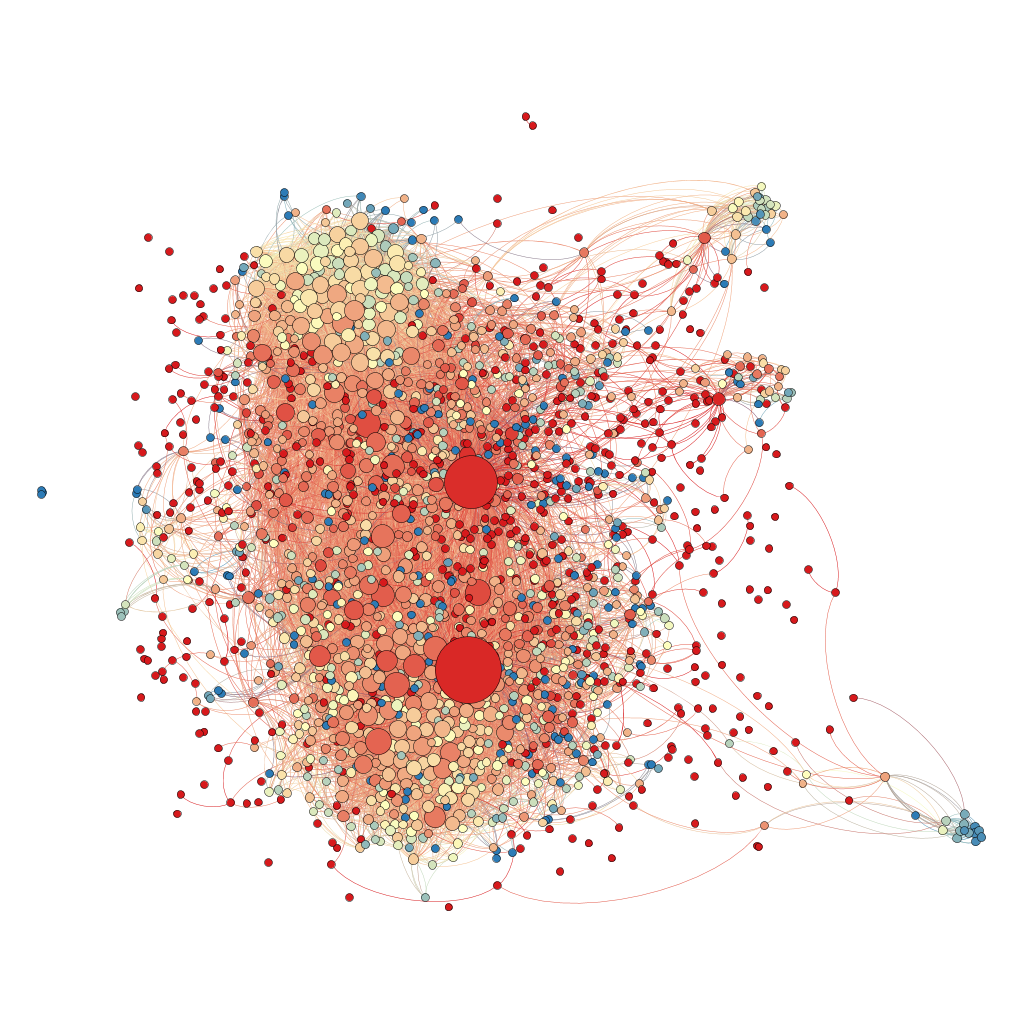
\includegraphics[scale=.25]{figs/Silicon}
% 	\caption{An example network image rendered from the Silicon Valley (Facebook) group using Gephi and the Force Atlas 2 layout algorithm.
% 	See Section~\ref{sec:gephi} for further information.}
% \label{fig:gephi}
% \begin{flushleft}\footnotesize
% Source: By the author.\
% \end{flushleft}
% \end{center}
% \end{figure}

\begin{figure}[!tbp]
	\centering
	    \subfloat[\footnotesize Without participant names.]{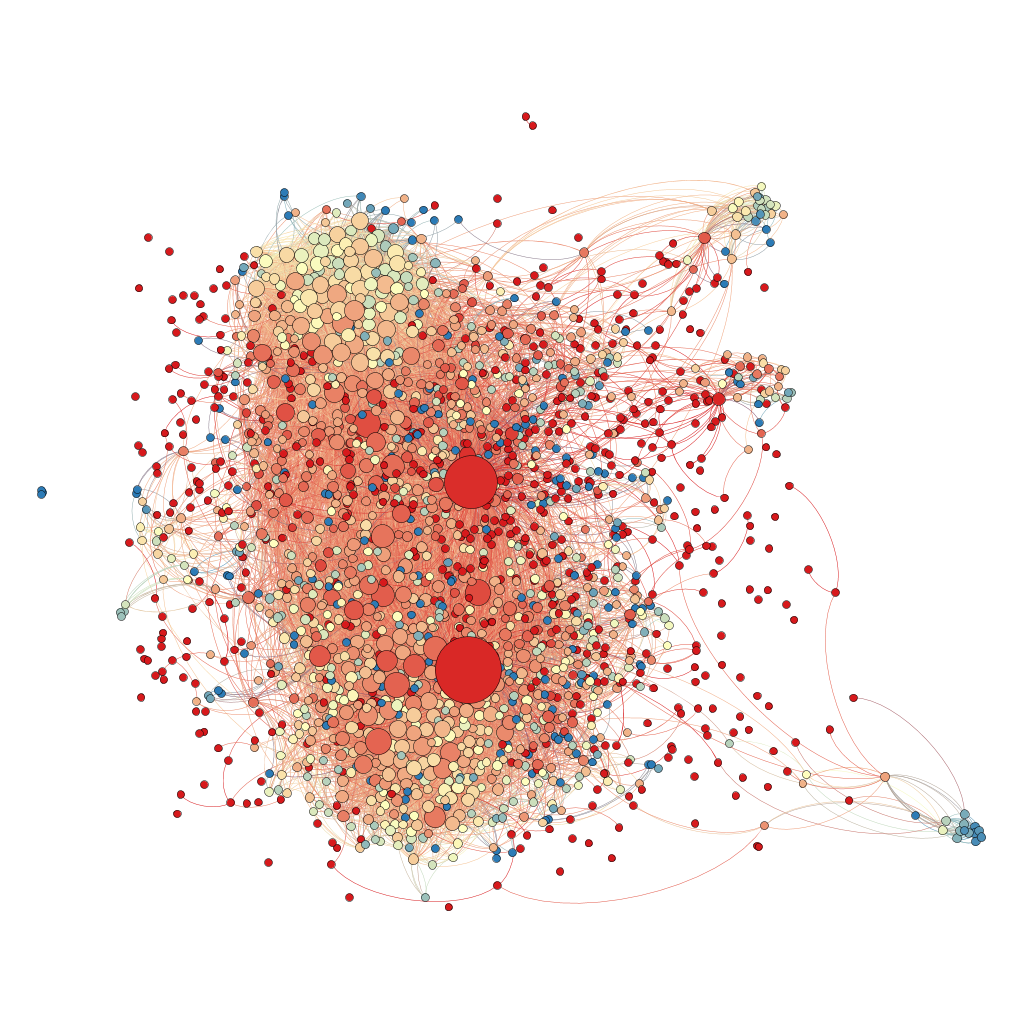
\includegraphics[width=0.45\textwidth]{figs/Silicon.png}\label{fig:f1}}
		\subfloat[\footnotesize With participant names.]{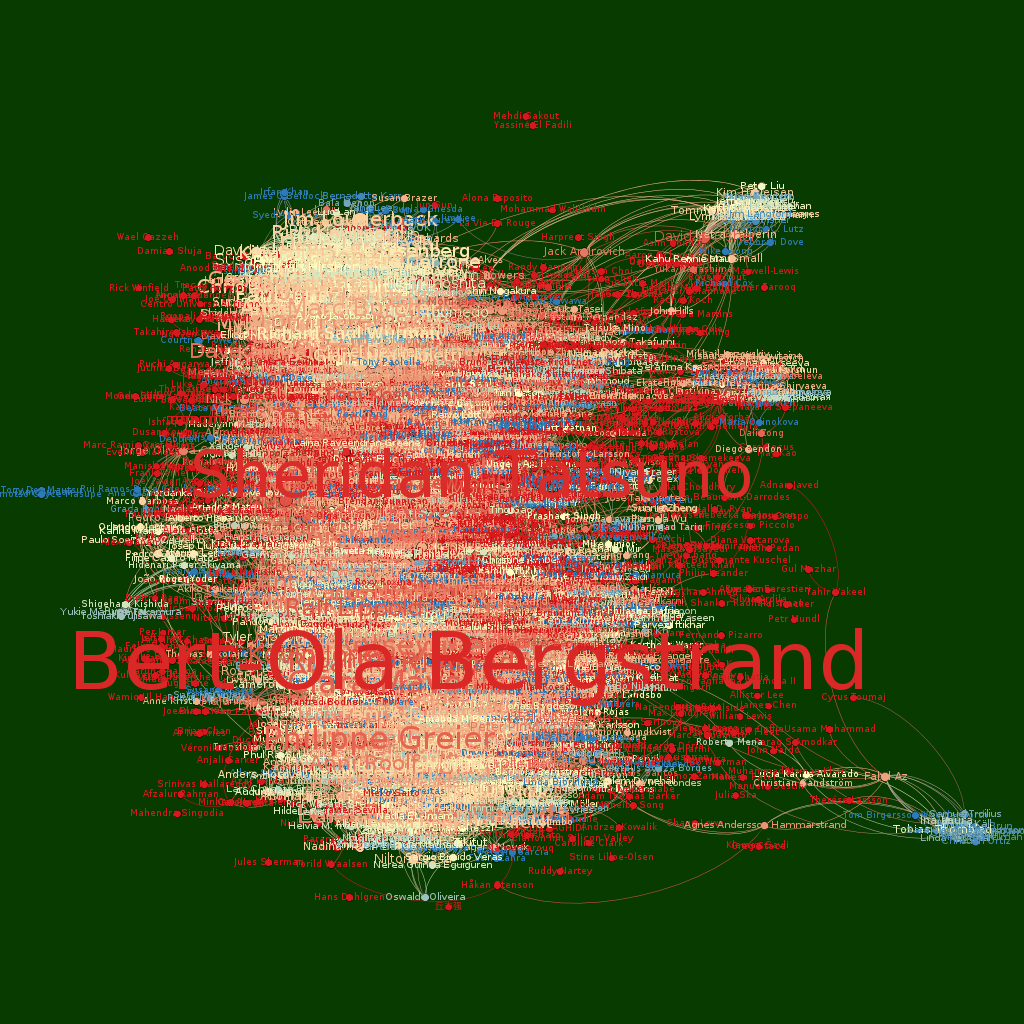
\includegraphics[width=0.45\textwidth]{figs/Silicon_nomes.png}\label{fig:f2}}
	\caption{An example network image rendered from the Silicon Valley (Facebook) group using Gephi and the Force Atlas 2 layout algorithm.
	See Section~\ref{sec:gephi} for further information.}\label{fig:gephi}
\begin{flushleft}\footnotesize
Source: By the author.\
\end{flushleft}
\end{figure}


% fb pelo gephi
	\subsection{Art by Pedro Paulo Rocha}
\section{Mega networks}
\section{Ubiquity of inequality: a simple model that explains why power laws are so frequently found in empirical data}
% arte pelo Pedro Paulo Rocha
\section{Social structures live streaming}
% telões de redes e de medidas de texto
% uso no arenaNETmundial e no ocupaGOV e outras ocasiões online
\section{Kolmogorov-Smirnov test systematic measurements}
\section{OPS: the Social Participation (OWL) Ontology}
\section{OPa: the ParticipaBR (OWL) Ontology}
\section{OntologiAA: the AA (OWL) Ontology}
\section{The Algorithmic Autoregulation software development methodology}
\section{Social Library Ontology and Social Library Vocabulary: OBS in OWL and VBS in SKOS}
% Conselhos, Foruns, Mesas Redondas, etc. Casos feitos com especialistas, casos feitos a partir de documentações
\section{Genesis of this work: complex social networks analysis by emails}
\section{United Nations Development Program consulting}
\subsection{Partnership with the Brazilian Presidency}
\subsection{Description of each product}
\section{Govern art}
\section{Ideal ideas: a physical modeling of the mind}
\section{Webpages}
% ARS, texto para pedro
\section{Collection and diffusion of information in social networks}\label{sec:colDif}
\subsection{Progressive network activation from peripherals to hubs}
\subsection{Instantaneous network activation by betweenness and closeness centralities}
\subsection{Massive tagging in Facebook and email crossposting}
\subsection{SERVDDCR online video conferences}
% processo dos periféricos aos hubs
% instantâneos pelos de maior betweenness e maior closeness
% coleta e difusão através da citação de várias pessoas e de crosspost
% SERVDDCR
\section{Anthropological physics}
The study of complex systems can be undertaken as a physics endeavor,
specially if complex networks and statistics are into play. When the complex
system is constituted by people, intriguing questions arise from diverse field such as math, ethics, and sociology. The “anthropological physics”is an approach to these scenarios that enables scientific research while resolving ethical and moral issues by an open study of the self.
	It yields a transdisciplinary practice whose relevance emanate from anthropological
and physical matters, from human constituted systems and natural laws.
A sweet spot was found in recent civil, government and academic efforts~\cite{opa,ensaio}, and has been called anthropological physics. General characteristics are:
\begin{itemize}
	\item Exposure of the researcher to the environment of interest, such as virtual social networks.
	\item Use of the annotations from the exposure, be them activity logs, friendship or interaction networks, textual contents, etc.
	\item Upon need, expansion of observations to encompass open datasets or data donated by partners.
	\item Observance of natural laws as they appear in network structures and natural language.
	\item All resources are kept as open and publicized as possible, including software, data, and writings.
\end{itemize}                                                                                                                                     
A short report the first insights regarding anthropological physics is on~\cite{anPhy}.
 
% conceitualização básica, artigo e conferências
\section{Listing of documents written, conferences attended and artistic presentations}
% rcpln
% artigos
% conferências: duas nexos+ccdc+linguística+sifiscs+ufpa+
% apresentações na SGPR, imersões, arenaNETmundial
% vivace

\end{apendicesenv}


% ----------------------------------------------------------
% Anexos
% ----------------------------------------------------------
%% USPSC-Anexos.tex
% ---
% Inicia os anexos
% ---
\begin{anexosenv}

% Imprime uma página indicando o início dos anexos
\partanexos

% ---
\chapter{Exemplo de anexo}
% ---
Elemento opcional, que consiste em um texto ou documento não elaborado pelo autor, que serve de fundamentação, comprovação e ilustração, conforme a ABNT NBR 14724. \cite{nbr14724}.

O \textbf{ANEXO B} exemplifica como incluir um anexo em pdf.

\chapter{Acentuação (modo texto - \LaTeX)}
\begin{figure}[H]
	\begin{center}
	\caption{\label{fig_anexob}Acentuação (modo texto - \LaTeX)}
	\includegraphics[scale=1.0]{USPSC-AcentuacaoLaTeX.png} \\
	Fonte: \citeonline{comandos}
	\end{center}	
\end{figure}

\chapter{Símbolos úteis em \LaTeX}
\begin{figure}[H]
	\begin{center}
		\caption{\label{fig_anexoc}Símbolos úteis em \LaTeX}
		\includegraphics[scale=1.0]{USPSC-SimbolosUteis.png} \\
		Fonte: \citeonline{comandos}
	\end{center}	
\end{figure}


\chapter{Letras gregas em \LaTeX}
\begin{figure}[H]
	\begin{center}
		\caption{\label{fig_anexod}Letras gregas em \LaTeX}
		\includegraphics[scale=1.0]{USPSC-LetrasGregas.png} \\
		Fonte: \citeonline{comandos}
	\end{center}	
\end{figure}

\end{anexosenv}


%---------------------------------------------------------------------
% INDICE REMISSIVO
%--------------------------------------------------------------------
\phantompart
\printindex

%---------------------------------------------------------------------

\end{document}
